\documentclass[12pt]{article}
\usepackage{hyperref}
\usepackage[warn]{mathtext}
\usepackage[T2A]{fontenc}
\usepackage[utf8]{inputenc}
\usepackage[russian]{babel}
\usepackage{cite}
\usepackage{amsfonts}
\usepackage{lineno}
\usepackage{subfig}
\usepackage{graphicx}
\usepackage{xcolor}
\usepackage{bm}
\usepackage{graphicx}
\usepackage{amssymb}
\usepackage{hyperref}
\usepackage[left=2cm,right=2cm,top=2cm,bottom=2cm]{geometry}

\DeclareGraphicsExtensions{.png,.jpg,.svg,.pdf}
\author{Карцев Вадим}
\title{Лабораторная работа 5.6

Измерение $\beta$-спектров с помощью сцинтилляционного пластикового детектора}

\begin{document}

  \maketitle

  \textbf{Цель работы:} Хз

  \textbf{В работе используются:} Сцинтилляционный пластиковый детектор частиц,
  кюветы с источниками излучения ($^{137}Cs$, $^{90}Sr$, $^{36}Cl$, $^{60}Co$,
  $^{22}Na$), монета.

  \section{Теоретическая справка}

  \newpage
  \section{Обработка данных для $^{137}Cs$}

    \begin{figure}[h!]
      \begin{minipage}[h]{0.99\linewidth}
        \center{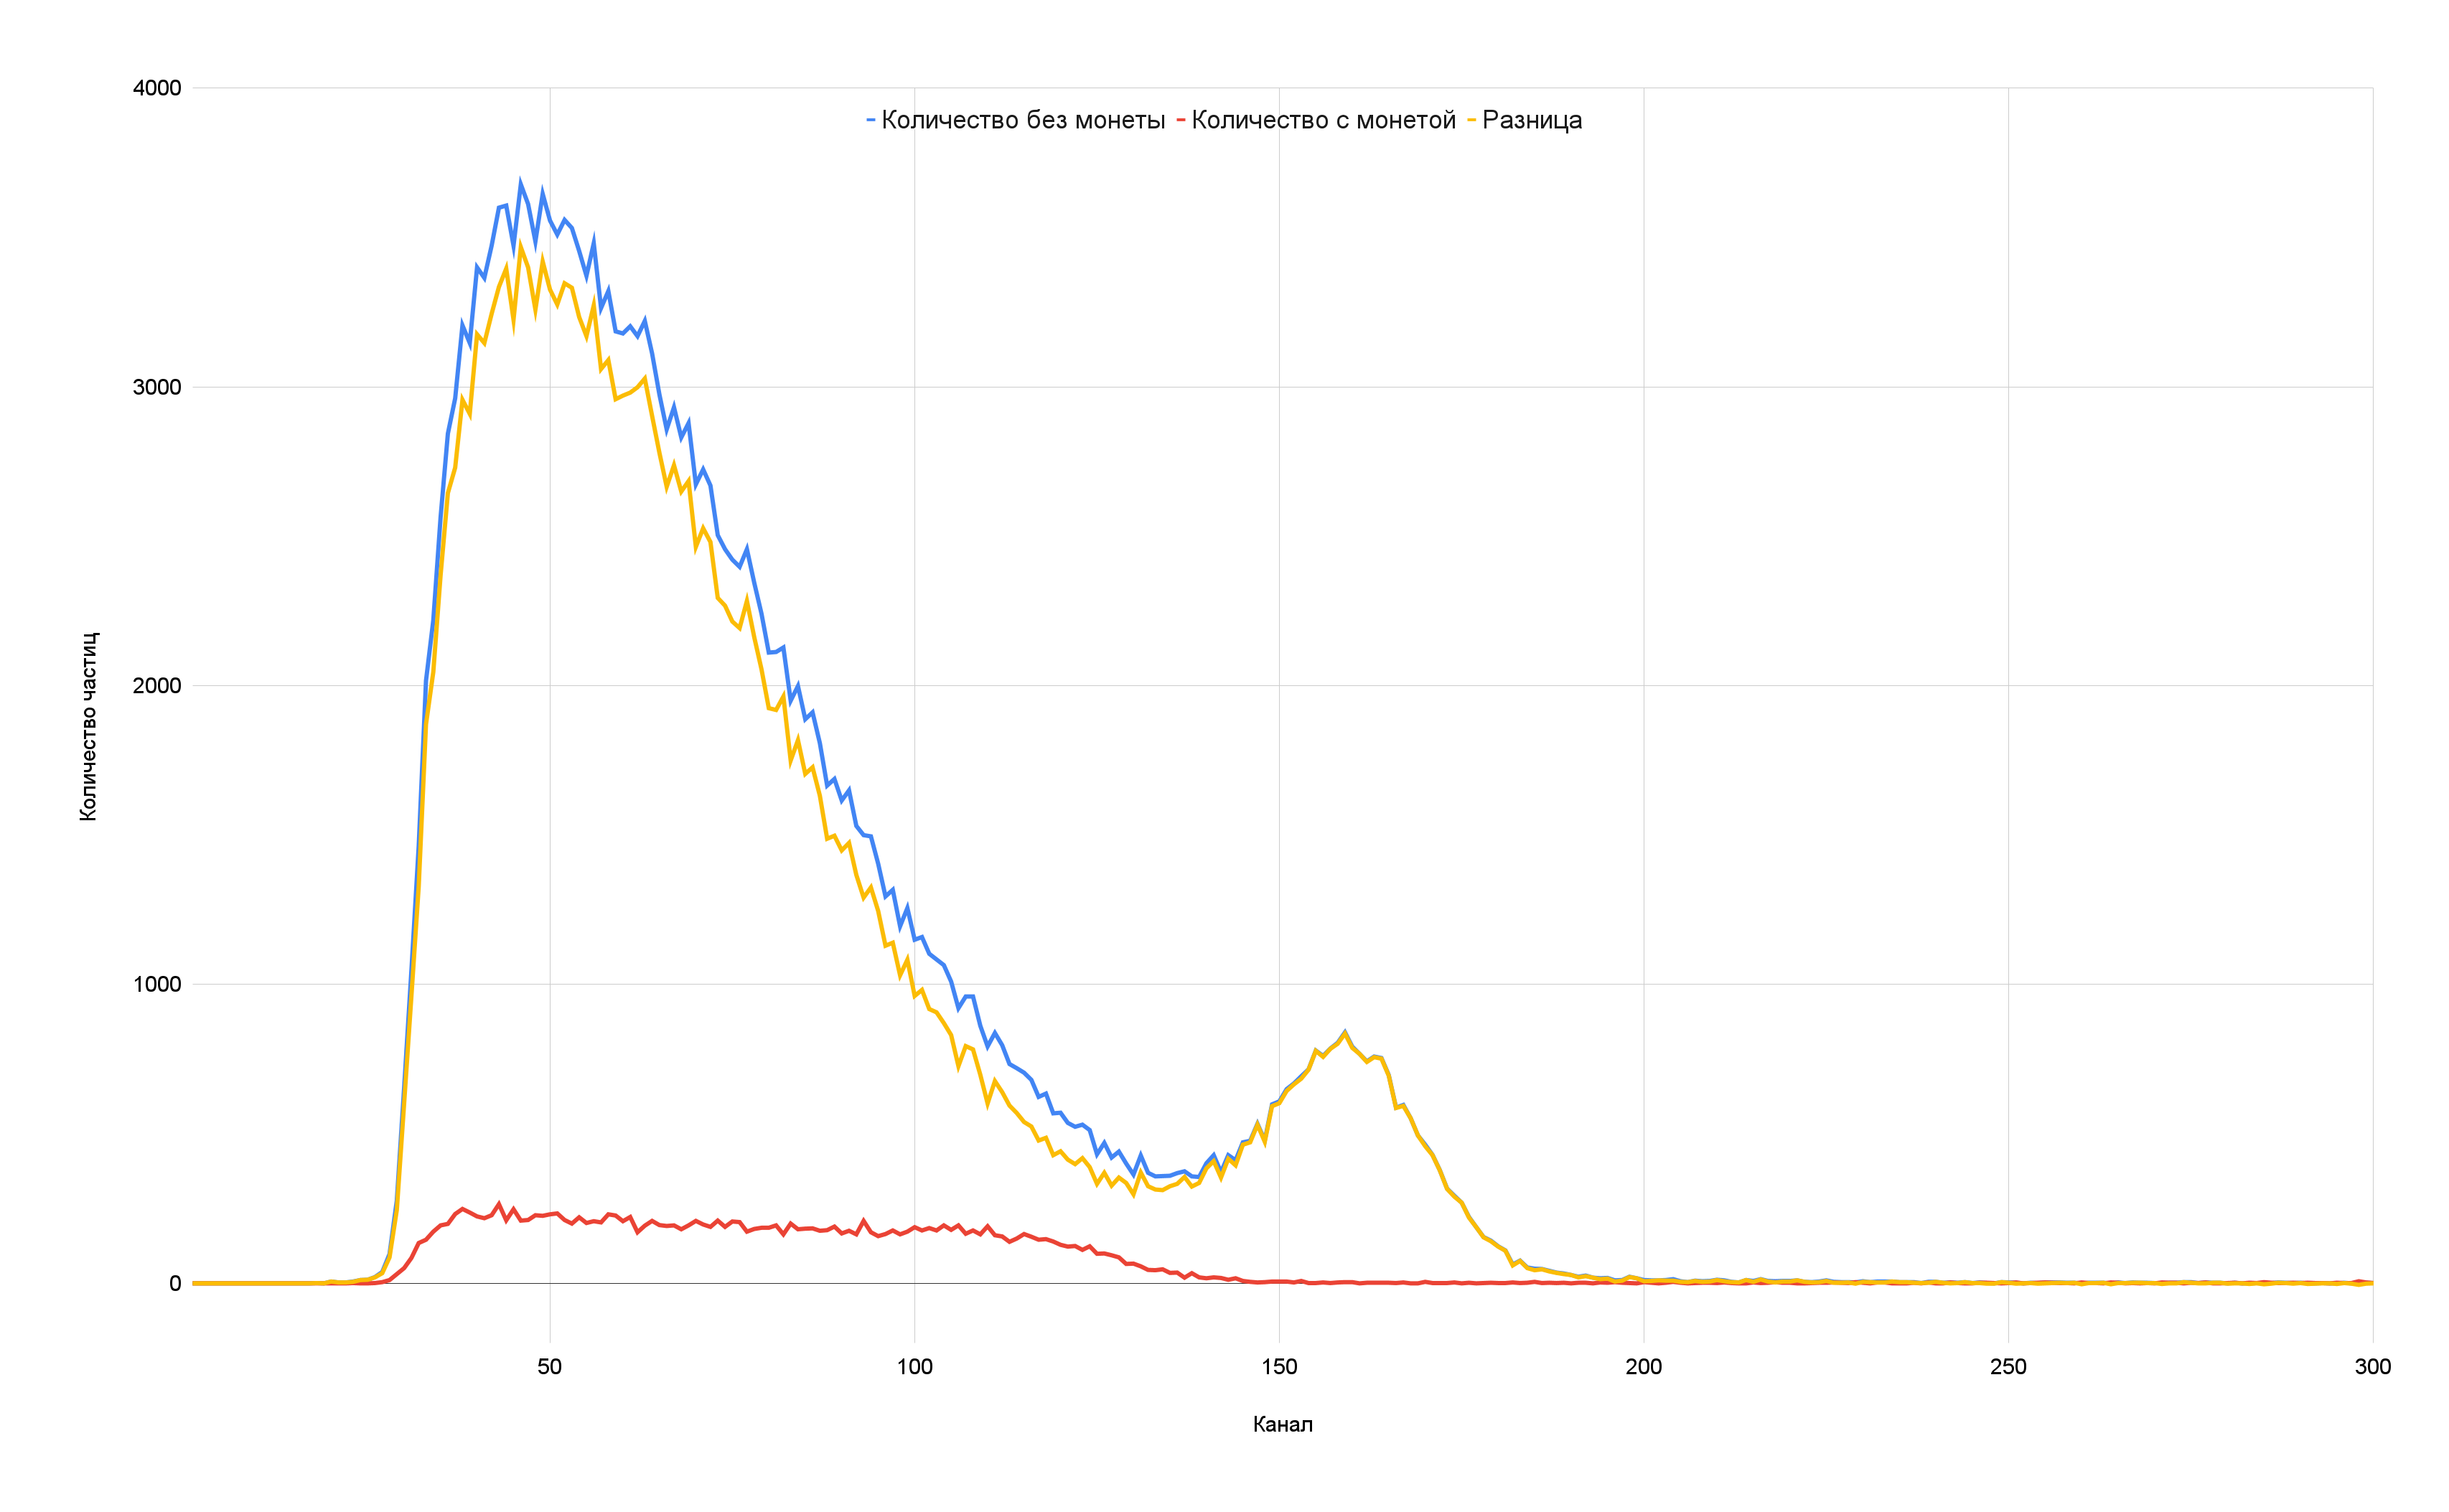
\includegraphics[width=0.99\linewidth]{cesium.png}}
        Рис 1. Спектры для цезия без монеты и с монетой, разница спектров
      \end{minipage}
      \label{chart:cesium}
    \end{figure}

  \newpage
  \section{Обработка данных для $^{90}Sr$}

    \begin{figure}[h!]
      \begin{minipage}[h]{0.99\linewidth}
        \center{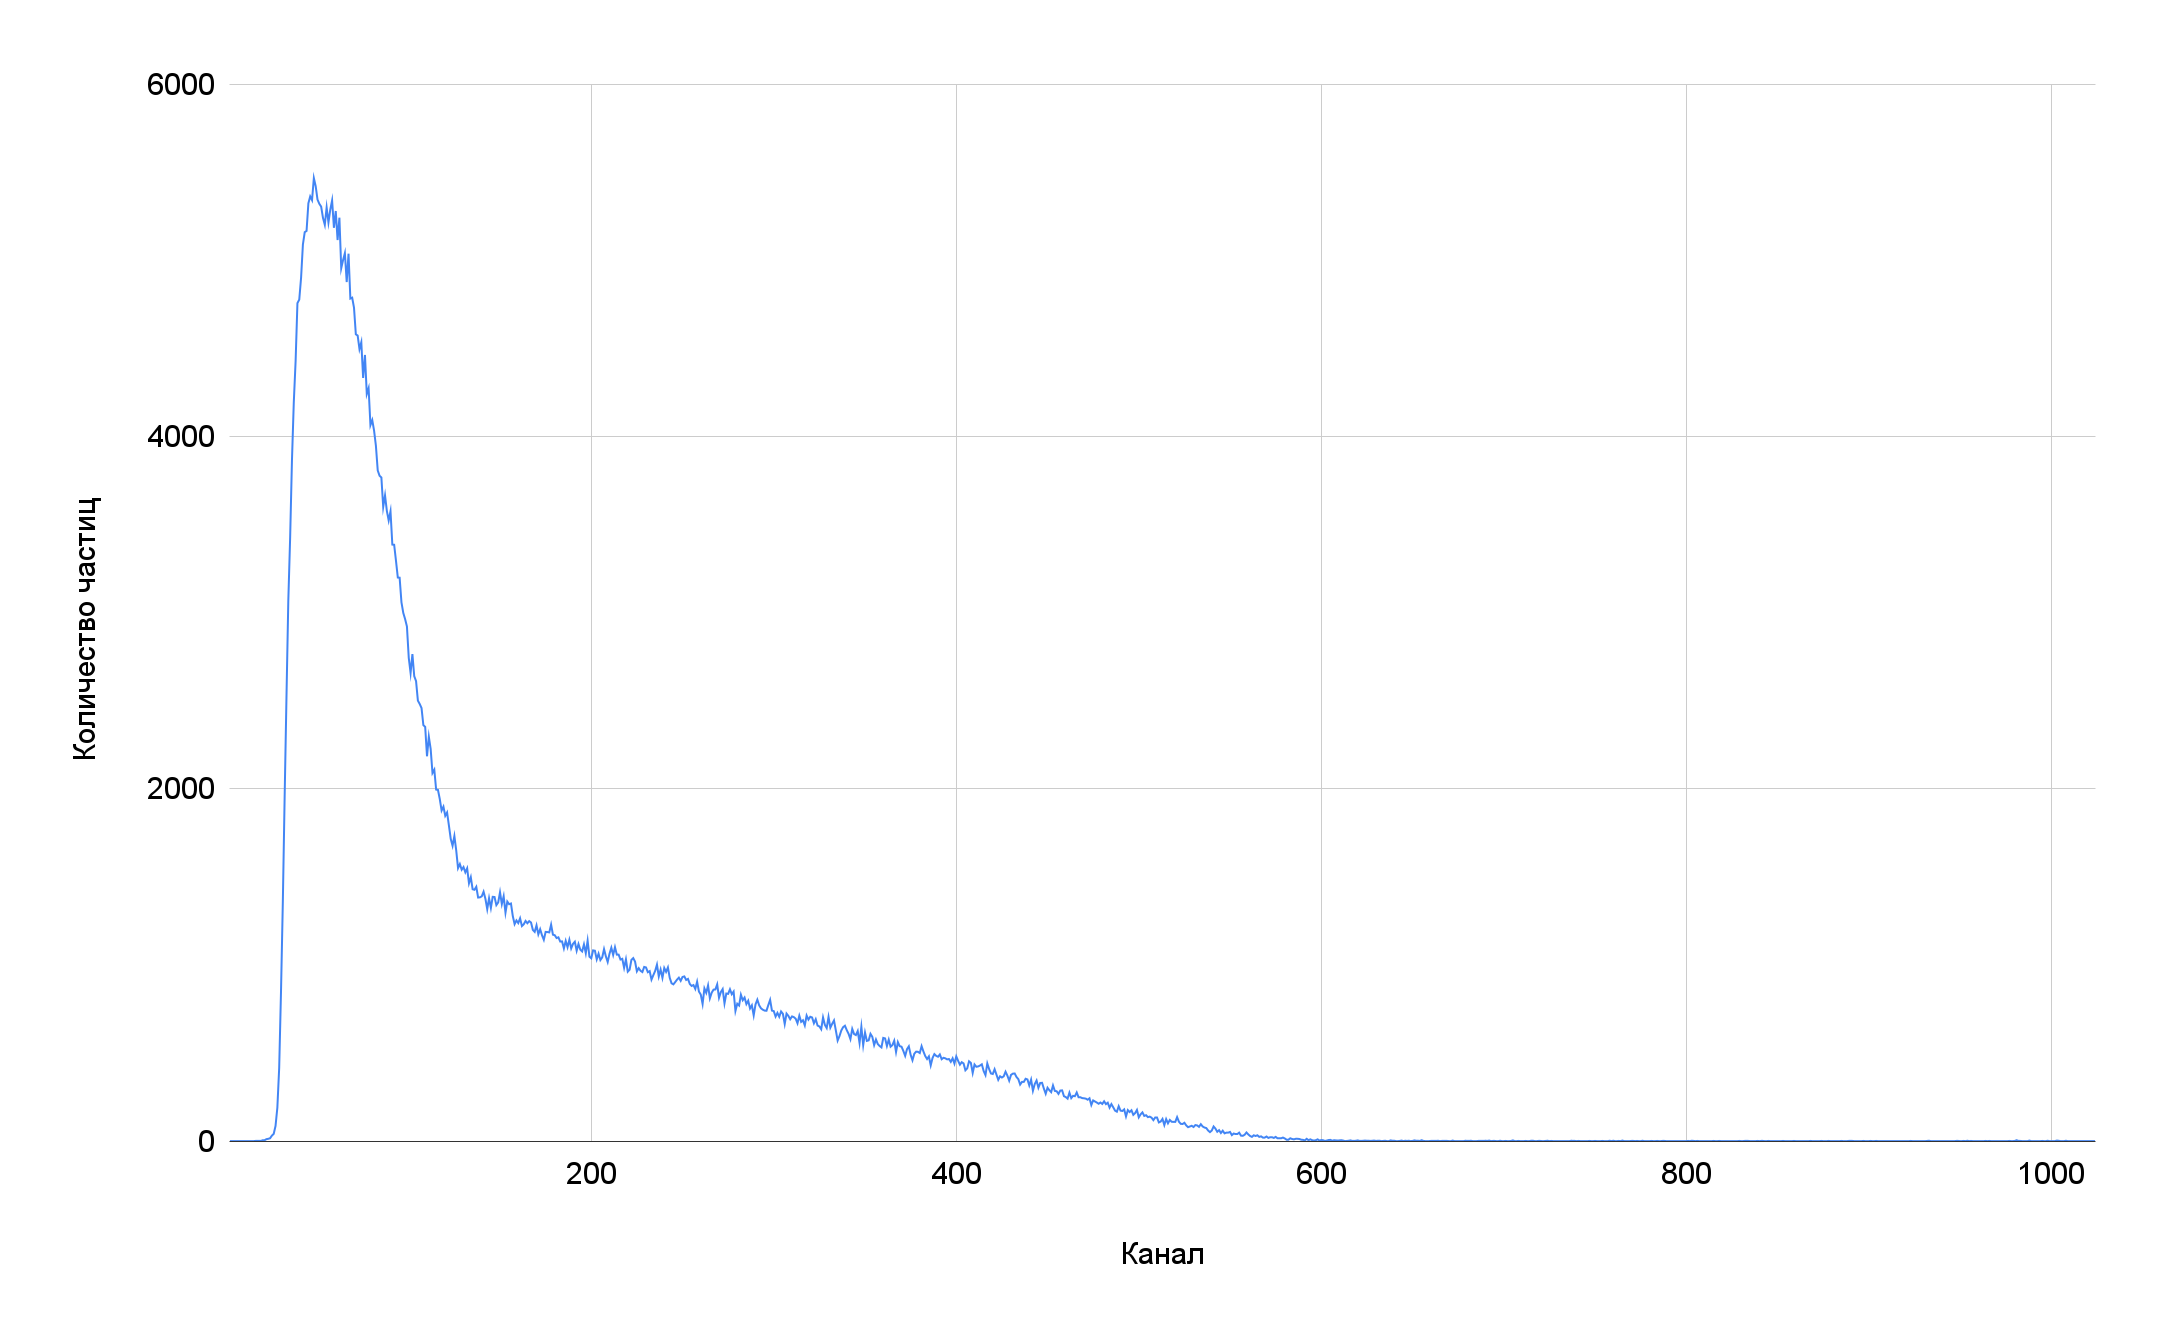
\includegraphics[width=0.99\linewidth]{strontium.png}}
        Рис 2. Спектр для стронция
      \end{minipage}
      \label{chart:strontium}
    \end{figure}

  \newpage
  \section{Обработка данных для $^{36}Cl$}

    \begin{figure}[h!]
      \begin{minipage}[h]{0.99\linewidth}
        \center{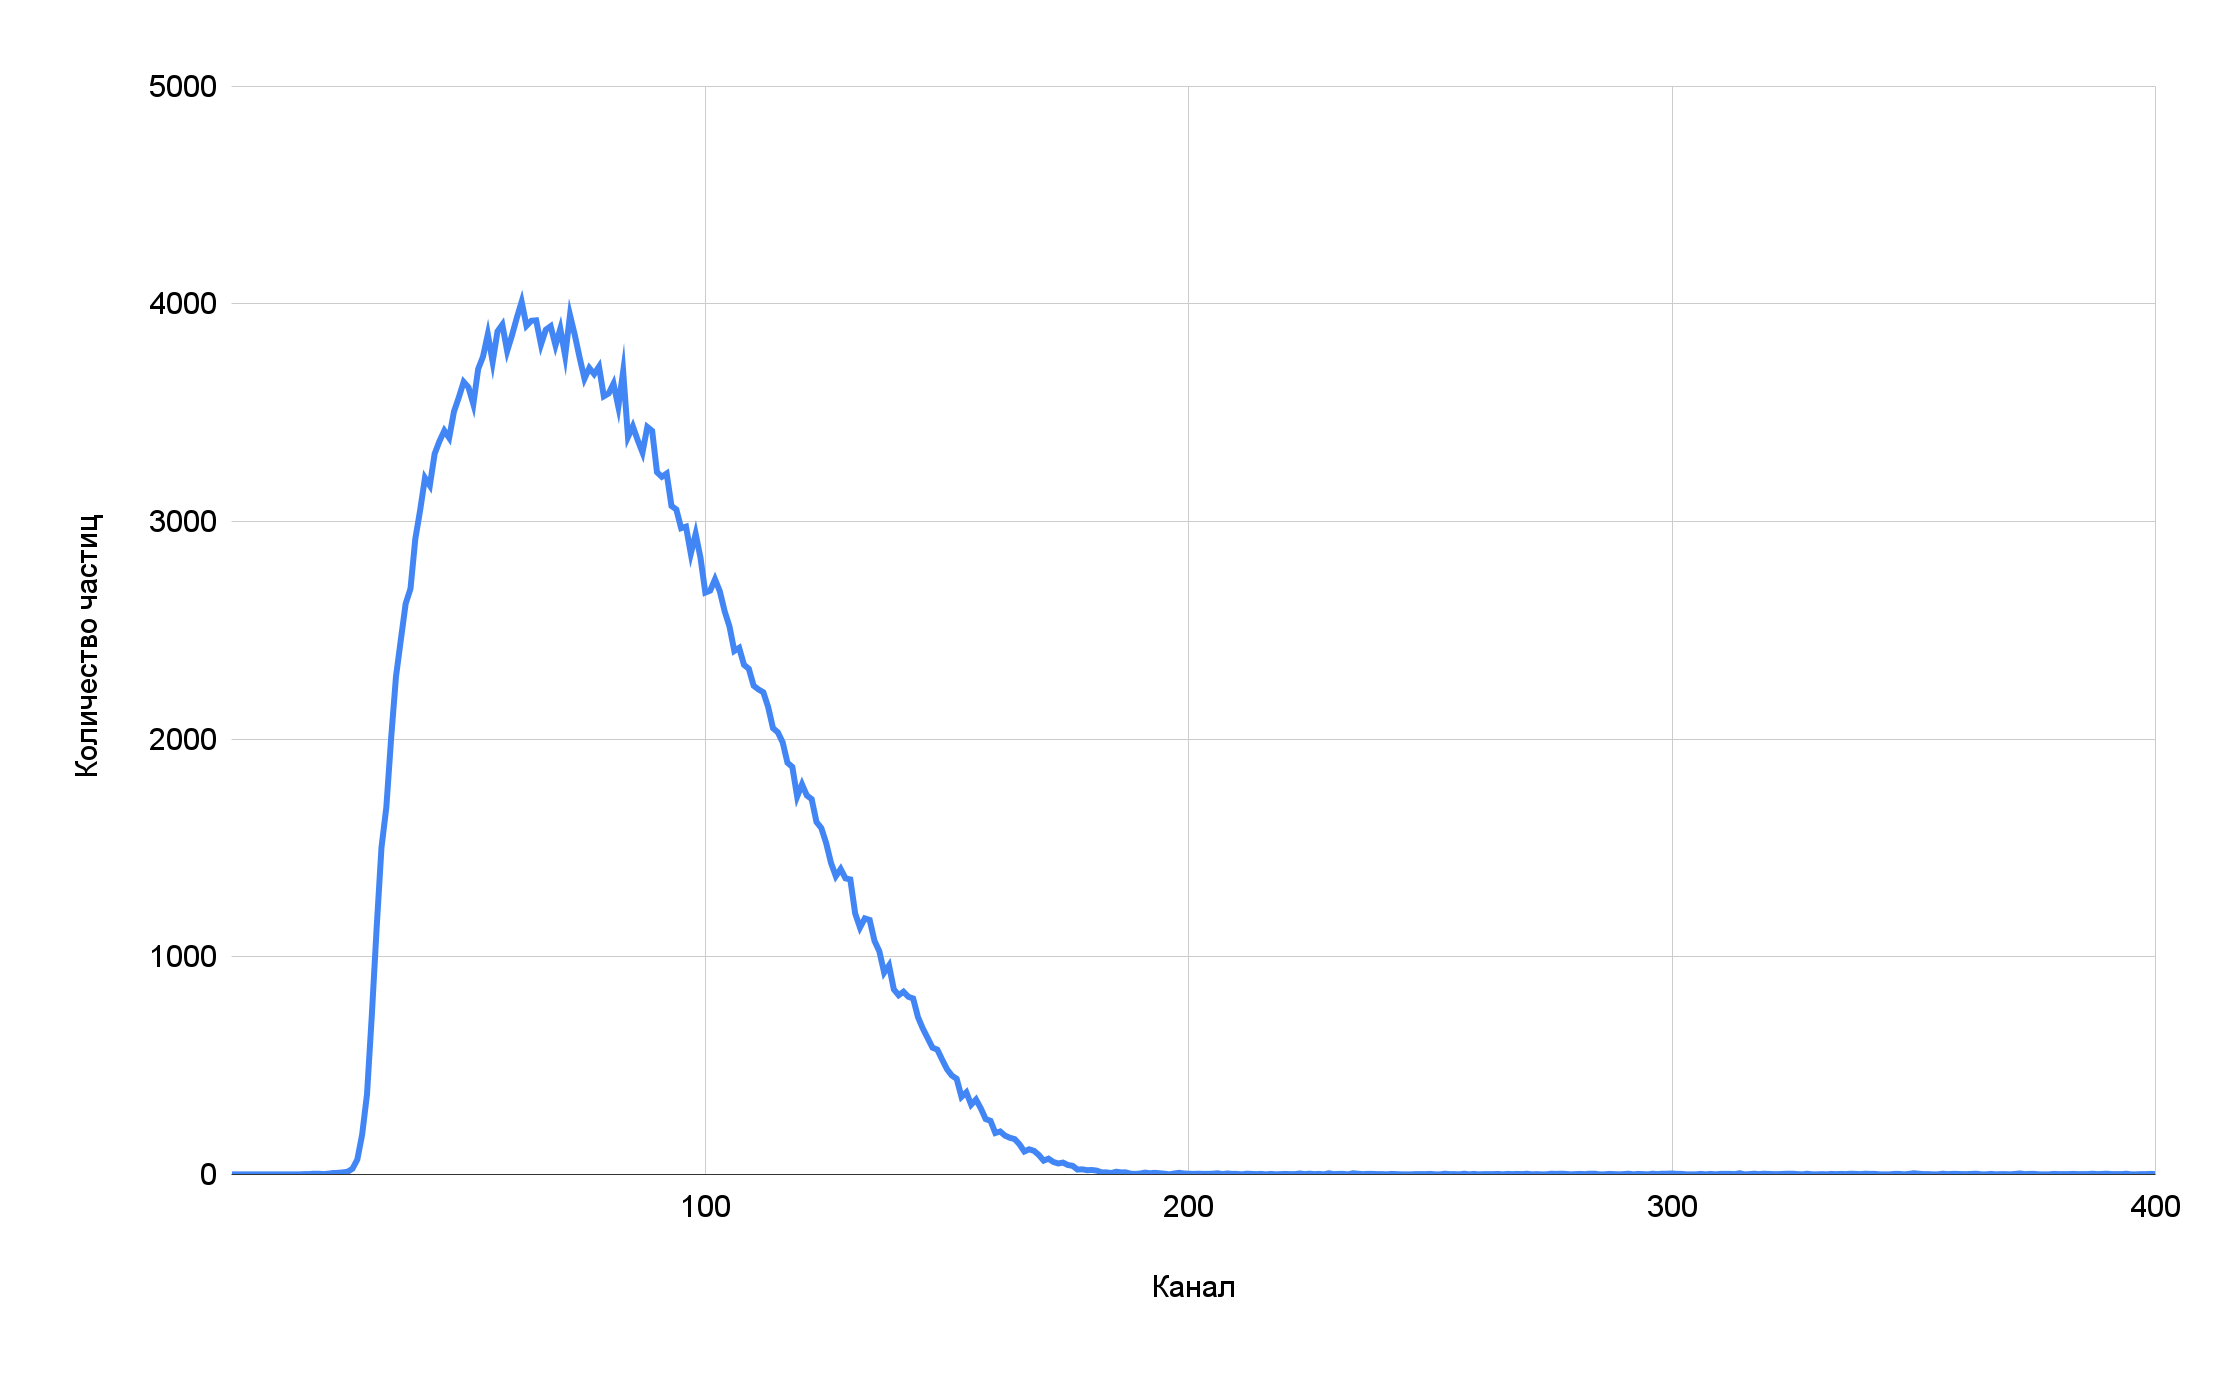
\includegraphics[width=0.99\linewidth]{chlorine.png}}
        Рис 3. Спектр для хлора
      \end{minipage}
      \label{chart:chlorine}
    \end{figure}

  \newpage
  \section{Обработка данных для $^{60}Co$}

    \begin{figure}[h!]
      \begin{minipage}[h]{0.99\linewidth}
        \center{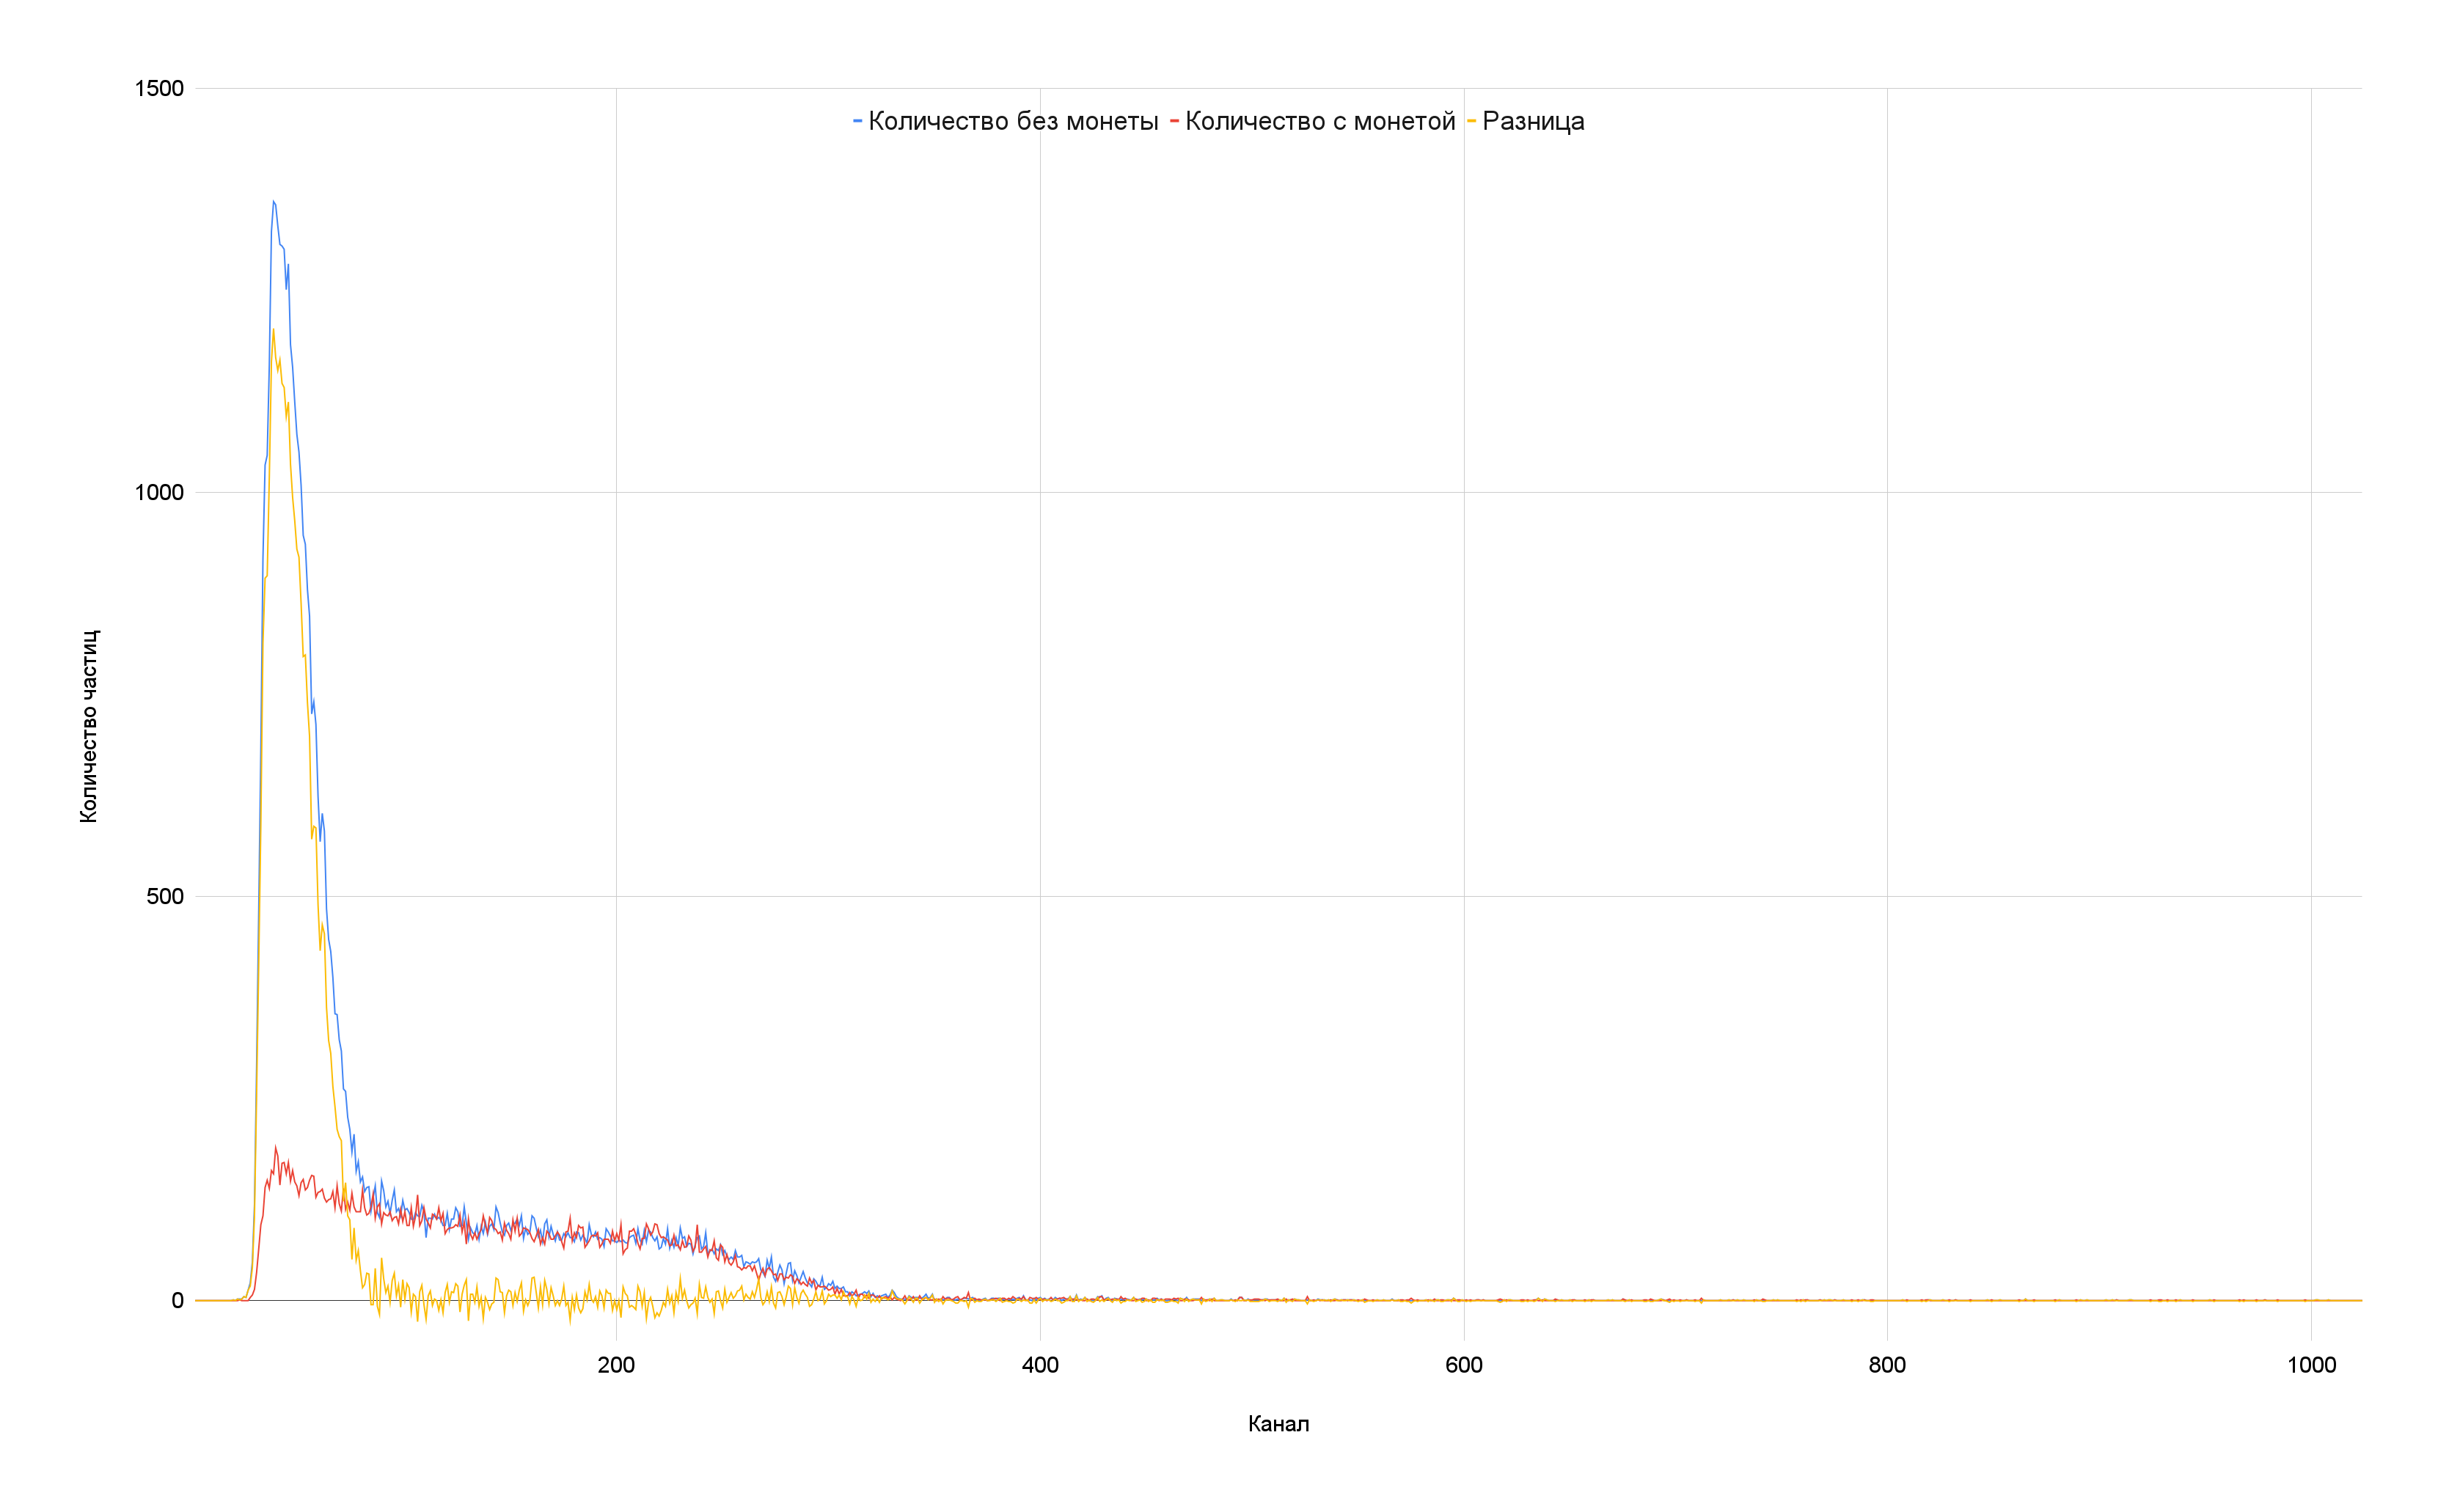
\includegraphics[width=0.99\linewidth]{cobalt.png}}
        Рис 4. Спектры для кобальта без монеты и с монетой, разница спектров
      \end{minipage}
      \label{chart:cobalt}
    \end{figure}

  \newpage
  \section{Обработка данных для $^{22}Na$}

    \begin{figure}[h!]
      \begin{minipage}[h]{0.99\linewidth}
        \center{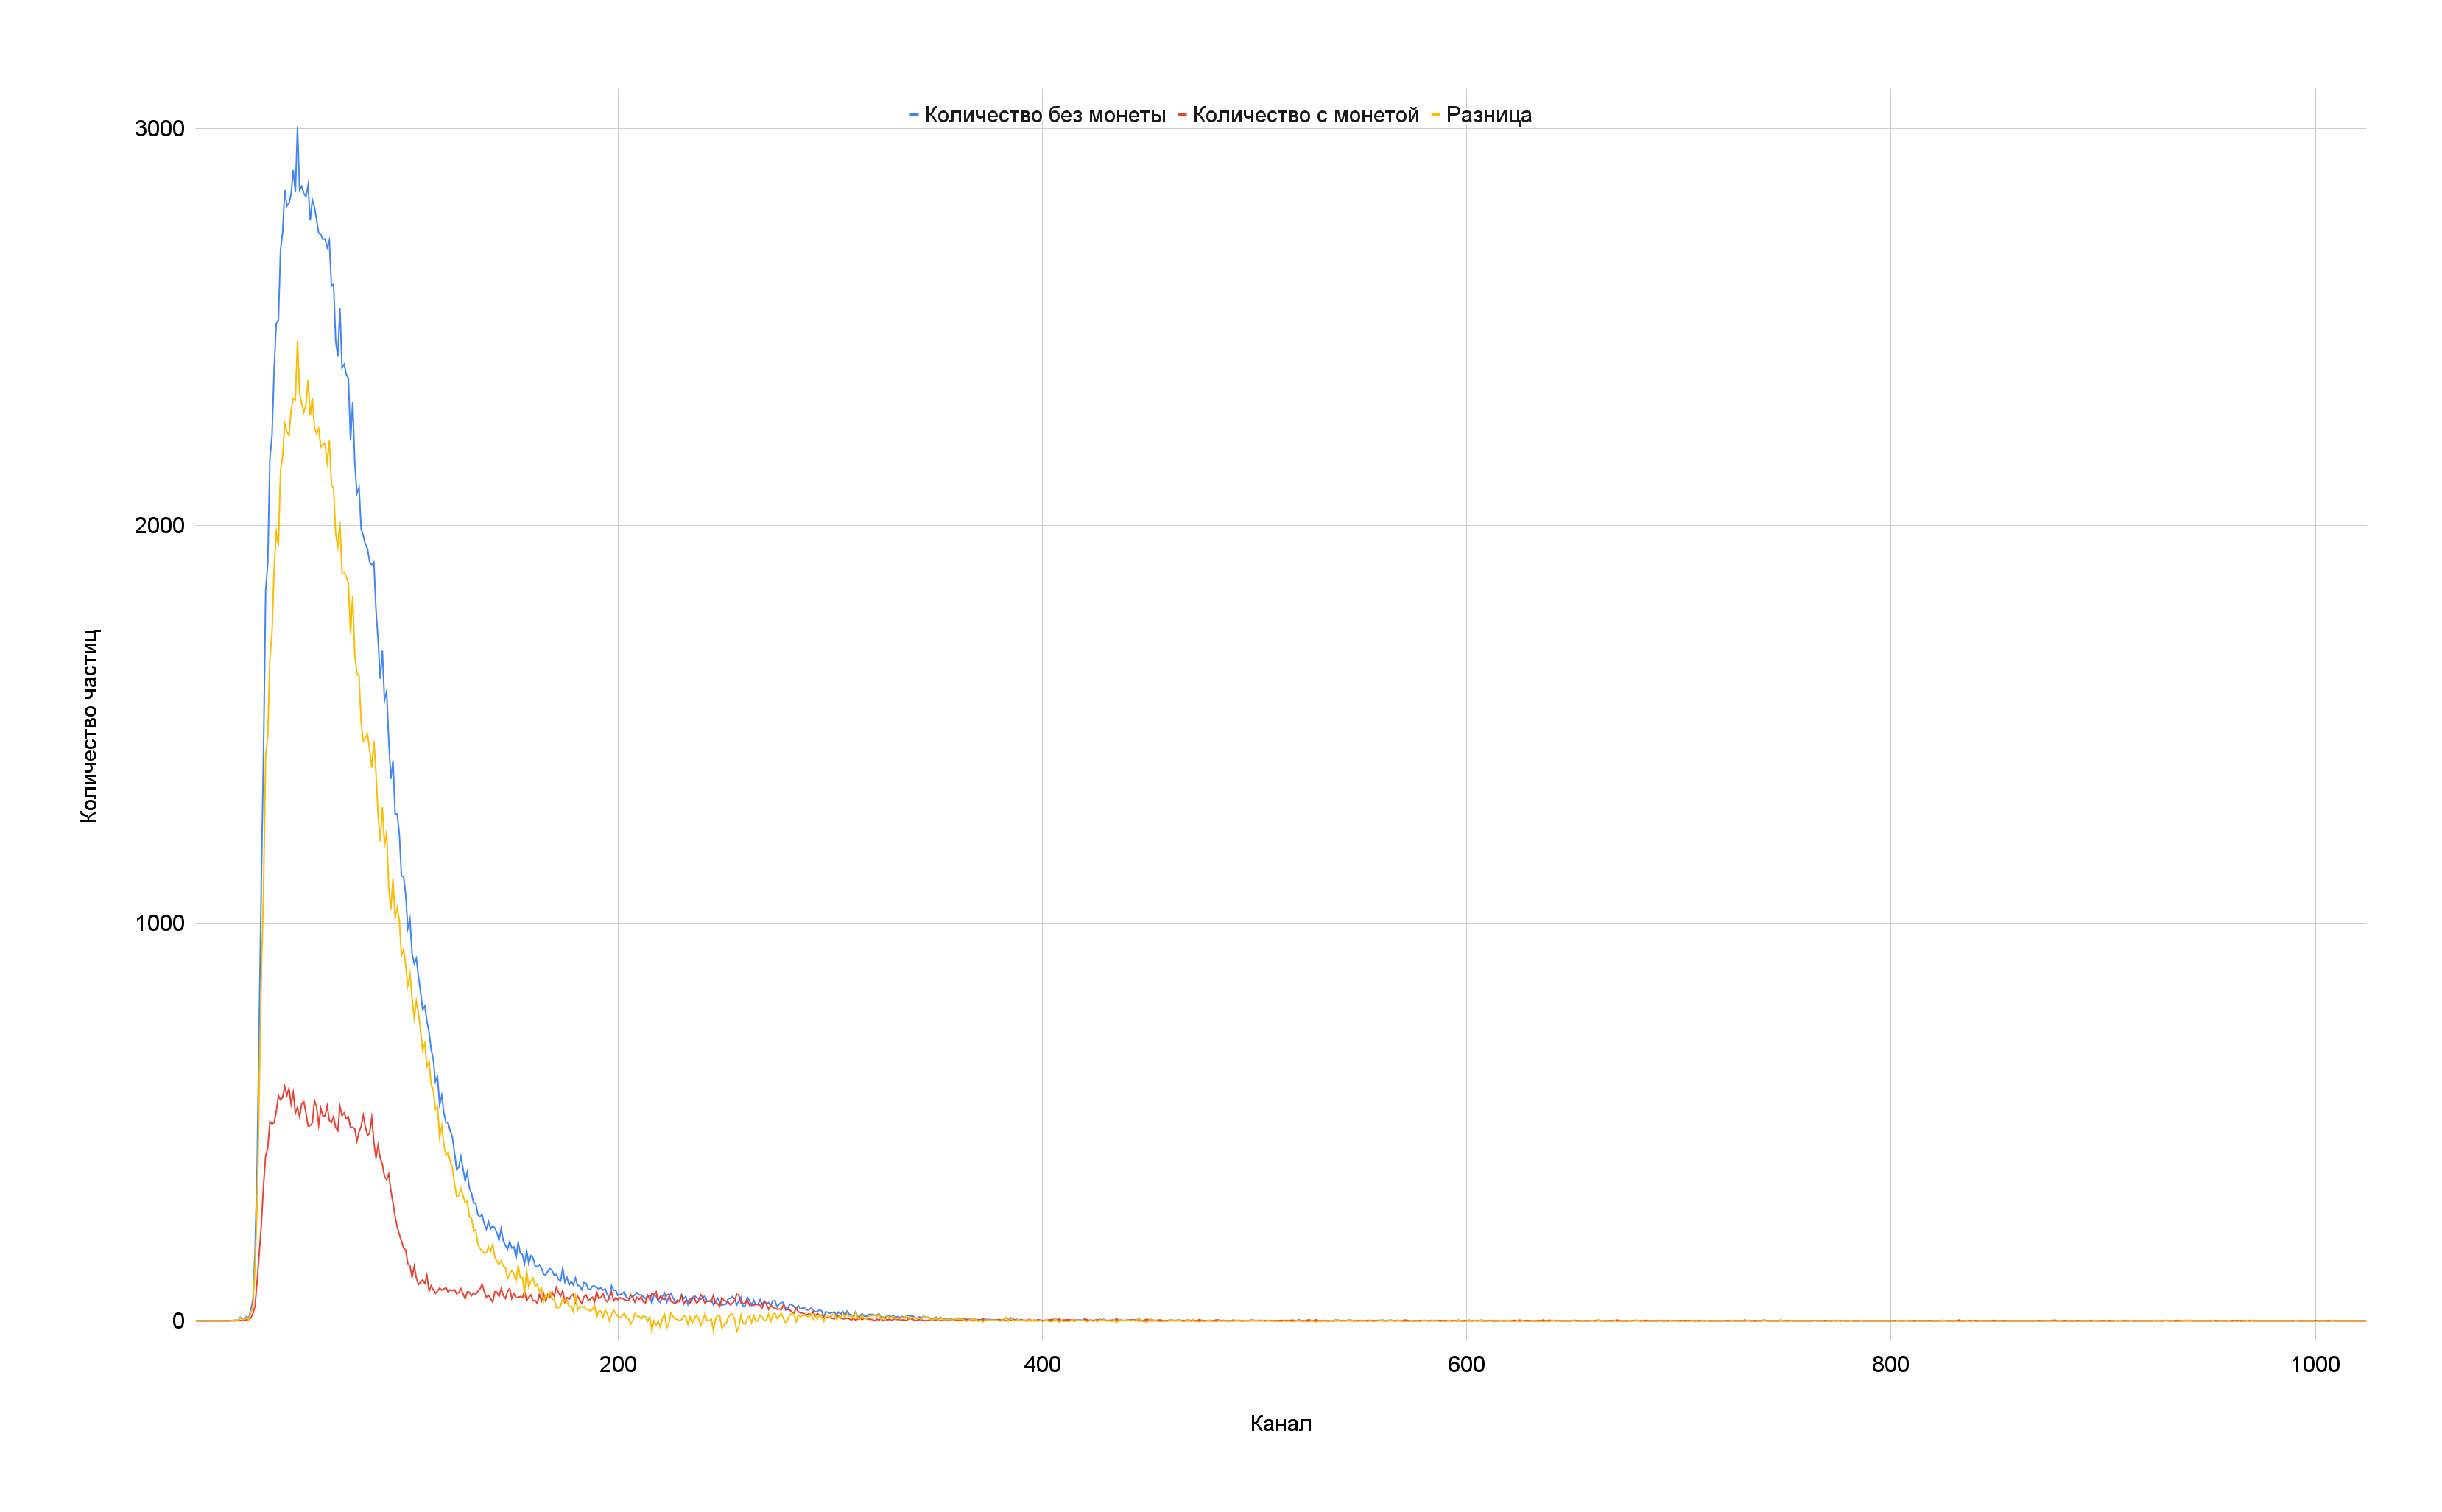
\includegraphics[width=0.99\linewidth]{natrium.png}}
        Рис 5. Спектры для натрия без монеты и с монетой, разница спектров
      \end{minipage}
      \label{chart:natrium}
    \end{figure}

  \newpage
  \section{Вывод}

\end{document}
